\capitulo{5}{Aspectos relevantes del desarrollo del proyecto}

En esta sección se van a detallar los aspectos más relevantes que han ido surgiendo a lo largo del desarrollo del proyecto. Este ha sido un desarrollo \textit{software} y como tal ha estado lleno de retos y decisiones técnicas que han tenido que ir tomándose. La formación ha sido un punto de inflexión, sumado a la aplicación de buenas prácticas, ha resultado en un producto de calidad.


\section{Investigación}
Uno de los componentes principales que posee el proyecto es el apartado de investigación en el campo del Aprendizaje Automático, concretando un poco más, el efecto de la aplicación de técnicas de selección de instancias en el aprendizaje semi-supervisado.

Uno de los principales retos a los que el autor se ha enfrentado en una primera instancia ha sido adquirir una rápida capacidad de lectura y asimilación de documentación científica, si bien el idioma (inglés) no ha supuesto una barrera, el no poseer experiencia en realizar estas tareas  generó una necesidad que tuvo que ser solventada poco a poco. En los últimos meses del proyecto la agilidad ya estaba ahí, resultando en tareas más fluidas y veloces.

\section{Metodología SCRUM}
Como ya se mencionó en la Sección~\ref{SCRUM}, el proyecto se ha realizado siguiendo una metodología ágil, permitiendo trabajar en \textit{sprints} de manera que el trabajo de cada \textit{sprint} se encuentre correctamente fundamentado al inicio de cada uno, permitiendo trabajar con una mayor eficiencia, priorizar el trabajo en función las tareas existentes, y disponer de versiones funcionales a la vez que se sigue con el desarrollo del proyecto.

Si bien se conocía SCRUM de manera puramente teórica, el haber trabajado siguiendo esta metodología ha permitido ganar experiencia en modelos de desarrollo ágiles, diferente de los clásicos a los que se acostumbraba, y tal y como se define, el trabajo se ha visto afectado de forma positiva con esta aproximación.

Se disponían de cerca de 9 meses (máximo) para cumplimentar el proyecto, un tiempo mucho más elevado del habitual para este tipo de proyectos, es por ello por lo que se han invertido múltiples \textit{sprints} para validación y calidad, permitiendo asegurar que los pasos dados son correctos y seguir construyendo sobre seguro.

Una de las principales dificultades encontradas en este campo es la asignación de puntos de historia, el definir en base a un nombre de tarea y una descripción el tiempo que va a ser necesario invertir para cumplir con ella no ha sido siempre muy preciso. El no poseer experiencia previa en proyectos de esta envergadura propició que se considerara la equivalencia de 1 punto de historia igual a 45 minutos o menos. Y si bien ha habido múltiples \textit{sprints} en los cuales se ha conseguido seguir esta relación, no ha sido algo lineal en el proyecto, debido a que se tuvo en cuenta la experiencia que se iba consiguiendo a la hora de asignar los siguientes puntos de historia, y ha habido múltiples \textit{sprints} desfasados por lo alto.

\section{Actualización y modificación de un \textit{software} pre-existente}
Posiblemente será el aspecto relevante más cercano a el futuro laboral de cualquier alumno. Supuso todo un reto el coger un proyecto que había sido desarrollado por 5 personas y <<hacerlo propio>>. Como es lógico cada persona programa de una forma diferente para alcanzar la misma funcionalidad, y ya no solo eso, sino la propia temática del proyecto era desconocida, por lo tanto, supuso un esfuerzo doble.

La no existencia de una documentación, ni técnica ni formal, acerca del propio \textit{software} no ayudó a obtener una visión del proyecto más allá de la estructura de paquetes y nombres. Fue algo que se echó en falta, y que, con la finalización de este proyecto, ya posee.

\section{Desarrollo Web}
A lo largo del Grado no se ha recibido docencia en cuanto a desarrollo web se refiere, siendo toda una desventaja a la hora de actualizar y modificar \texttt{UBUMLaaS}. Trabajar con una REST API era algo hasta enero desconocido, y la curva de aprendizaje no ha sido especialmente sencilla. Han sido necesarias numerosas horas para familiarizarse tanto con el proyecto como con la forma de trabajo que poseen las aplicaciones que siguen esta arquitectura.

A la hora de integrar nuevas modificaciones sobre el \textit{backend} del proyecto no supuso grandes problemas, fue un trabajo laborioso como es de esperar, pero al ser Python ya se estaba acostumbrado al lenguaje de programación. La dificultad llegó con el \textit{frontend}, lenguajes de marcas como HTML o CSS, y de programación como JavaScript, no eran desconocidos, pero no se habían utilizado nunca en grandes proyectos; es por ello por lo que hubo tareas que se vieron retrasadas. 

Hay que destacar que como ha sido la tónica general del proyecto, y así queda recogido en el resumen de numerosos \textit{sprints} en su anexo correspondiente, a medida que el equipo de desarrollo se familiarizaba con el lenguaje y entorno de aplicación, la velocidad de implementación de funcionalidades crecía de forma exponencial.

La web ha sufrido una renovación completa, siendo necesario re-escribir todos los documentos HTML, si bien se tuvo desde un inicio en cuenta que ciertas páginas tuvieran un diseño similar al que ya poseían anteriormente para seguir con el diseño inicial. El nuevo diseño soporta múltiples resoluciones de pantalla, habiendo sido priorizadas aquellas soportadas en tabletas sobre las de dispositivos móviles.

\subsection{Funcionalidades <<sobre la marcha>>}
A lo largo del desarrollo de la parte de administración de \texttt{UBUMLaaS} surgían cada día nuevas funcionalidades que parecían correctas o adecuadas para implementar y añadir, permitiendo a los administradores tener más control del que iban a poseer una vez pase a producción la versión creada.

Muchas de estas nuevas funcionalidades se han llevado a cabo y se encuentran disponibles y completamente integradas con la plataforma, si bien muchas otras no, se han quedado como trabajos futuros. Aquellas que se han quedado sin implementar fueron clasificadas con una relevancia baja, siendo priorizadas aquellas que se consideraron más útiles o curiosas.

\section{PIP}
\texttt{IS-SSL} es una biblioteca desarrollada con la finalidad de que sea útil a la mayor cantidad de desarrolladores posible, siguiendo las directrices del \textit{Open Source}, es por ello por lo que se encuentra disponible a través del gestor de paquetes de Python, PIP. 

El proyecto también puede ser descargado directamente desde el repositorio de GitHub y realizar todas las instalaciones de dependencias necesarias a través del fichero de \texttt{requeriments.txt} o creando un entorno de \texttt{Conda} (a través del fichero \texttt{is-ssl.yml}).

\section{Docker}
\texttt{UBUMLaaS} se encuentra desplegado en la Universidad de Burgos sobre un servidor directamente, pero con el fin de permitir que se despliegue en cualquier equipo y que la configuración específica sea mínima, se ha creado un contenedor Docker en el cuál reside la última versión de la aplicación. 

El futuro de la aplicación podría ser únicamente en Docker perfectamente, siendo mucho más sencillo desplegarla en diferentes servidores, pero en la actualidad ese no es el enfoque deseado, por lo que se dejó para hacer al final en caso de que sobrara tiempo, como ha sucedido.

\section{Validación de la integridad de los algoritmos implementados}
Todos los algoritmos que se encuentran disponibles en \texttt{IS-SSL} han sido validados y refinados a lo largo de múltiples iteraciones de trabajo con el fin de garantizar su integridad, de forma que se puede asegurar que reportan resultados tal y como el \textit{paper} original lo presentó.

\begin{itemize}
\item Los algoritmos de selección de instancias han sido validados contra los homónimos correspondientes proporcionados por \texttt{Weka}.
\item Los algoritmos de aprendizaje semi-supervisado han sido validados contra los implementados por el grupo de investigación ADMIRABLE de la Universidad de Burgos.
\end{itemize}


\section{Experimentación de filtros de ruido para aprendizaje semi-supervisado}
La problemática al utilizar algoritmos de SSL se presenta en forma de que numerosos estudios empíricos demuestran que existen situaciones en las cuales el uso de esos datos no etiquetados puede degradar el modelo. Siendo aconsejable el poder explotar los datos de forma segura.

Es por ello por lo que múltiples estudios~\cite{zhao2021safe, guo2020safe, li2016towards} ya se han adentrado en el aprendizaje semi-supervisado seguro. Entendiendo por \emph{seguro} que el rendimiento de la generalización nunca es estadísticamente peor que los métodos que sólo utilizan datos etiquetados~\cite{li2019safe}.

La experimentación llevada a cabo posee como objetivo validar la hipótesis:\\
\emph{<<¿Se obtiene un etiquetado más seguro en aprendizaje semi-supervisado gracias a la aplicación de métodos de selección de instancias en combinación con self-training?>>}.

Introduciendo como novedades nuevos métodos de selección de instancias, así como clasificadores, hasta ahora no evaluados en problemas de esta naturaleza.

\subsection{Experimentación}
La experimentación en una primera instancia ha sido realizada utilizando \textit{self-training}, como algoritmo de aprendizaje semi-supervisado, utilizando como clasificadores base: \textit{K-Nearest Neighbors} y árboles de decisión. 

En una segunda instancia se siguió la aproximación propuesta en~\cite{li2019selfk}, bajo la cual el etiquetado de las instancias se produce en base a picos de densidad y la reducción de este mediante el uso mediante el uso de un filtrado de ruido previo.

Para la realización de la experimentación se utilizan 18 conjuntos de datos seleccionados del repositorio de la Universidad de California Irvine (UCI), la descripción de los diferentes conjuntos de datos se encuentra en la Tabla~\ref{tab:exp:datasets}. Los experimentos son realizados con diferentes porcentajes de número de instancias etiquetadas sobre el total, disponibles en la Tabla~\ref{tab:exp:percents}.

En todos los experimentos, se realiza una validación cruzada de 10 \textit{folds}, con el fin de obtener los resultados de la experimentación se utilizan las métricas \textit{accuracy} (ACC), \textit{f1 score}, y el error cuadrático medio.

\begin{align}
\text{\textit{ACC}} & = \frac{\text{\# tp}}{\text{\# Total de instancias}} \\
\text{\textit{f1-score}} & = \frac{\text{\# tp}}{\text{\# tp} + \frac{1}{2}\left( \text{\# fp} + \text{\# fn}\right)} \\
\text{\textit{MSE}} & = \frac{1}{n} \sum_{i=1}^{n}\left(Y_i - Y_j\right)^2
\end{align}

\noindent Métricas alcanzadas a partir de la matriz de confusión, esta es una herramienta que permite analizar los resultados de cómo trabaja un algoritmo de aprendizaje automático, repartiendo la información en columnas con las predicciones realizadas y en filas para el número real de instancias de cada clase. 
Donde TP representa los \textit{true positive}, TN los \textit{true negative}, FP los \textit{false positives} y FN los \textit{false negatives}. 

El conjunto de datos es dividido en 10 \textit{folds}, 9 de ellos son usados como conjunto de entrenamiento y 1 para el conjunto de prueba/validación/\textit{test}. Se utiliza selección estratificada aleatoria para la separación de los datos en entrenamiento y validación.

Anteriores artículos~\cite{li2019selfk} proponen esta misma aproximación, pero utilizando únicamente el filtro propio \emph{ENaNE}, y el clasificador base \textit{k-Nearest Neighbors}, tal y como se muestra en la Tabla~\ref{tab:exp:classifiers}.

La aproximación propuesta en esta documentación utiliza 3 clasificadores base con el fin de obtener una mayor diversidad de soluciones. Además, se utilizan los métodos de selección de instancias presentados en la Tabla~\ref{tab:exp:filters}.
Con todo esto se obtiene un espectro mucho más amplio de soluciones comparables, permitiendo validar la hipótesis planteada.

El  procedimiento seguido es directo y sencillo, mediante el uso de una semilla aleatoria, se asegura que todos los clasificadores y filtros poseen los mismos datos en cada \textit{n-ésima} iteración. El pseudocódigo se encuentra disponible en el Algoritmo~\ref{alg:pseudo-exp}.

\begin{algorithm}[]
  $random\_seed \leftarrow XX$\\
  \For {dataset en datasets}{
		\For {clasificador en clasificadores}{
			\For {filtro en filtros}{
				\For {\textit{fold} en CV} {
				Instanciar el modelo con sus parámetros. \\
				Entrenar el modelo. \\
				Predecir los datos de test. \\
				Cálculo de métricas. \\
				Guardar las métricas.
				}
			}		
		}
	}
	\caption{Pseudocódigo del proceso de experimentación.}\label{alg:pseudo-exp}
\end{algorithm}

\begin{table}[]
    \centering
    \begin{tabular}{ll}
	\toprule
        \textbf{Clasificador base} & \textbf{Parámetros} \\ 
    \toprule
        \textit{k Nearest Neighbors} & \textit{k} = 3 \\
        \textit{Decision Tree} & \textit{criterion} = gini \\ 
        \textit{Gaussian NB} & ~ \\ 
    \bottomrule
    \end{tabular}
    \caption{Clasificadores base utilizados en la experimentación.}\label{tab:exp:classifiers}
\end{table}

\begin{table}[]
    \centering
    \begin{tabular}{llc}
	\toprule
        \textbf{Filtro} & \textbf{Parámetros} & \textbf{Referencia} \\ 
    \toprule
        \textit{ENN} & \textit{k-NN} = 3, \textit{distance function} = \textit{euclidean} & \cite{wilson1972asymptotic} \\
        \textit{LSSm} & ~ & \cite{leyva2015three} \\ 
        \textit{ENaNE} & ~ & \cite{li2019selfk} \\ 
    \bottomrule
    \end{tabular}
    \caption{Filtros utilizados en la experimentación.}\label{tab:exp:filters}
\end{table}

\begin{table}[]
    \centering
    \tiny
    \begin{tabular}{lrrrc}
		\toprule
        \textbf{Conjuntos de datos} & \textbf{Instancias} & \textbf{Atributos} & \textbf{Clases} & \textbf{Abreviación} \\ 
        \toprule
        User Knowledge Modeling & 403 & 5 & 5 & UKM \\ 
        Thoracic Surgery Data  & 470 & 16 & 2 & TSD \\
        SPECTF Heart & 267 & 44 & 2 & SPH \\
        Sonar & 208 & 60 & 2 & SON \\ 
        Image Segmentation & 2.310 & 19 & 7 & IMS \\ 
        Pendigits & 3.498 & 16 & 10 & PEN \\
        Liver  & 345 & 6 & 2 & LIV \\ 
        Ionosphere & 351 & 34 & 2 & ION \\
        Glass & 214 & 10 & 7 & GLA \\ 
        Ecoil & 336 & 7 & 8 & ECO \\ 
        Blood Transfusion Service Center & 748 & 4 & 2 & BTSC \\ 
        Dermatology  & 366 & 34 & 6 & DER \\
        Satimage & 6.435 & 36 & 7 & SAT \\ 
        Wireless Indoor Localization & 2.000 & 7 & 4 & WIL \\ 
        Wholesale Customers  & 440 & 7 & 2 & WHC \\ 
        Indian Liver Patient Data set & 583 & 10 & 2 & ILPD \\ 
        Breast Tissue & 106 & 9 & 6 & BRT \\ 
        Letter  & 15.534 & 16 & 26 & LET \\ 
        \bottomrule
    \end{tabular}
    \caption{Descripción de los conjuntos de datos usados en la experimentación.}\label{tab:exp:datasets}
\end{table}

\begin{table}[]
    \centering
    \tiny
    \begin{tabular}{lrrrrrrr|r}
    \toprule
        \textbf{Conjunto de datos} & \textbf{5\%} & \textbf{10\%} & \textbf{15\%} & \textbf{20\%} & \textbf{25\%} & \textbf{30\%} &\textbf{ 35\%} & \textbf{100\%} \\ 
    \toprule
        UKM & 20 & 40 & 60 & 80 & 100 & 120 & 141 & 403 \\ 
        TSD & 23 & 47 & 70 & 94 & 117 & 141 & 164 & 470 \\ 
        SPH & 13 & 26 & 40 & 53 & 66 & 80 & 93 & 267 \\
        SON & 10 & 20 & 31 & 41 & 52 & 62 & 72 & 208 \\ 
        IMS & 115 & 231 & 346 & 462 & 577 & 693 & 808 & 2.310 \\ 
        PEN & 174 & 349 & 524 & 699 & 874 & 1.049 & 1.224 & 3.498 \\ 
        LIV & 17 & 34 & 51 & 69 & 86 & 103 & 120 & 345 \\ 
        ION & 17 & 35 & 52 & 70 & 87 & 105 & 122 & 351 \\ 
        GLA & 10 & 21 & 32 & 42 & 53 & 64 & 74 & 214 \\
        ECO & 16 & 33 & 50 & 67 & 84 & 100 & 117 & 336 \\
        BTSC & 37 & 74 & 112 & 149 & 187 & 224 & 261 & 748 \\ 
        DER & 18 & 36 & 54 & 73 & 91 & 109 & 128 & 366 \\
        SAT & 321 & 643 & 965 & 1.287 & 1.608 & 1.930 & 2.252 & 6.435 \\ 
        WIL & 100 & 200 & 300 & 400 & 500 & 600 & 700 & 2.000 \\ 
        WHC & 22 & 44 & 66 & 88 & 110 & 132 & 154 & 440 \\ 
        ILPD & 29 & 58 & 87 & 116 & 145 & 174 & 204 & 583 \\ 
        BRT & 5 & 10 & 15 & 21 & 26 & 31 & 37 & 106 \\ 
        LET & 776 & 1.553 & 2.330 & 3.106 & 3.883 & 4.660 & 5.436 & 15.534 \\ 
        \bottomrule
    \end{tabular}
    \caption{Relación del número de instancias de cada conjunto de datos con los diferentes porcentajes de etiquetado utilizados.}\label{tab:exp:percents}
\end{table}

\FloatBarrier
\subsection{Resultados}
El análisis de los resultados a los que podemos llegar se realiza en función de cada estimador base, ya que se han seleccionado 3 de naturaleza distinta, no se pueden comparar de manera directa entre ellos.

La aproximación seguida para conocer qué filtro (si es que existe) reporta mejores resultados para cada conjunto: estimador base-filtro, han sido los \textit{rankings} medios; se han evaluado para cada conjunto de datos y cada porcentaje de etiquetado. En la Figura~\ref{fig:exp-general} se muestra un resumen de todos los filtros para cada estimador\footnote{\emph{base} hace referencia a el resultado reportado por el estimador sin la aplicación de ningún método de selección de instancias sobre el conjunto de datos etiquetados.}. 

\imagenRuta{../img/memoria/aspectos-relevantes/General}{Resumen en función del clasificador y filtro.}{exp-general}

En la Figura~\ref{fig:exp-general} no se aprecia a <<simple vista>> tendencia alguna para ningún clasificador base y método de selección de instancias, que destaque sobre el resto. Si bien se puede intuir que \texttt{LSSm} tiende a mejorar según se poseen más instancias etiquetadas, no se puede asegurar a priori, es por ello por lo que se realizan tests estadísticos para comprobar si existen diferencias significativas entre los mismos.

El cálculo de los \textit{rankings} medios se ha validado gracias al uso de la herramienta \texttt{KEEL}\footnote{\textit{Knowledge Extraction based on Evolutionary Learning}. Herramienta de software Java que puede utilizarse para un gran número de tareas diferentes de descubrimiento de datos de conocimiento. KEEL proporciona una sencilla interfaz gráfica de usuario basada en el flujo de datos para diseñar experimentos con diferentes conjuntos de datos y algoritmos de IA.}~\cite{alcala2009keel, alcala2011keel}. Con la verificación de que los cálculos son correctos, se procede a realizar el \textit{test} de Nemenyi~\cite{nemenyi1963distribution} como \textit{test} \textit{post-hoc}, con el objetivo de encontrar las diferencias significativas entre clasificadores y los filtros utilizados. Este último paso viene propiciado como resultado de que el \textit{test} de Friedman~\cite{friedman1937use} rechazara la hipótesis nula.

Por motivos de espacio se muestra un resumen de las figuras obtenidas: \ref{fig:knn-posthoc}, \ref{fig:gaussnb-posthoc} y \ref{fig:tree-posthoc},  cada par clasificador-porcentaje de instancias etiquetadas dispone de su propio diagrama de \emph{Critical Difference} disponibles desde el siguiente \href{https://github.com/dpr1005/Semisupervised-learning-and-instance-selection-methods/tree/main/experimentation/result_plots}{enlace}. De igual manera los \texttt{CSVs} resultantes del proceso de experimentación, los \textit{logs}, los \textit{rankings} medios, \dots, se encuentran disponibles en el correspondiente directorio del \href{https://github.com/dpr1005/Semisupervised-learning-and-instance-selection-methods/tree/main/experimentation}{repositorio} de \texttt{IS-SSL}.

\begin{figure*}
        \centering
        \begin{subfigure}[b]{0.475\textwidth}
            \centering
            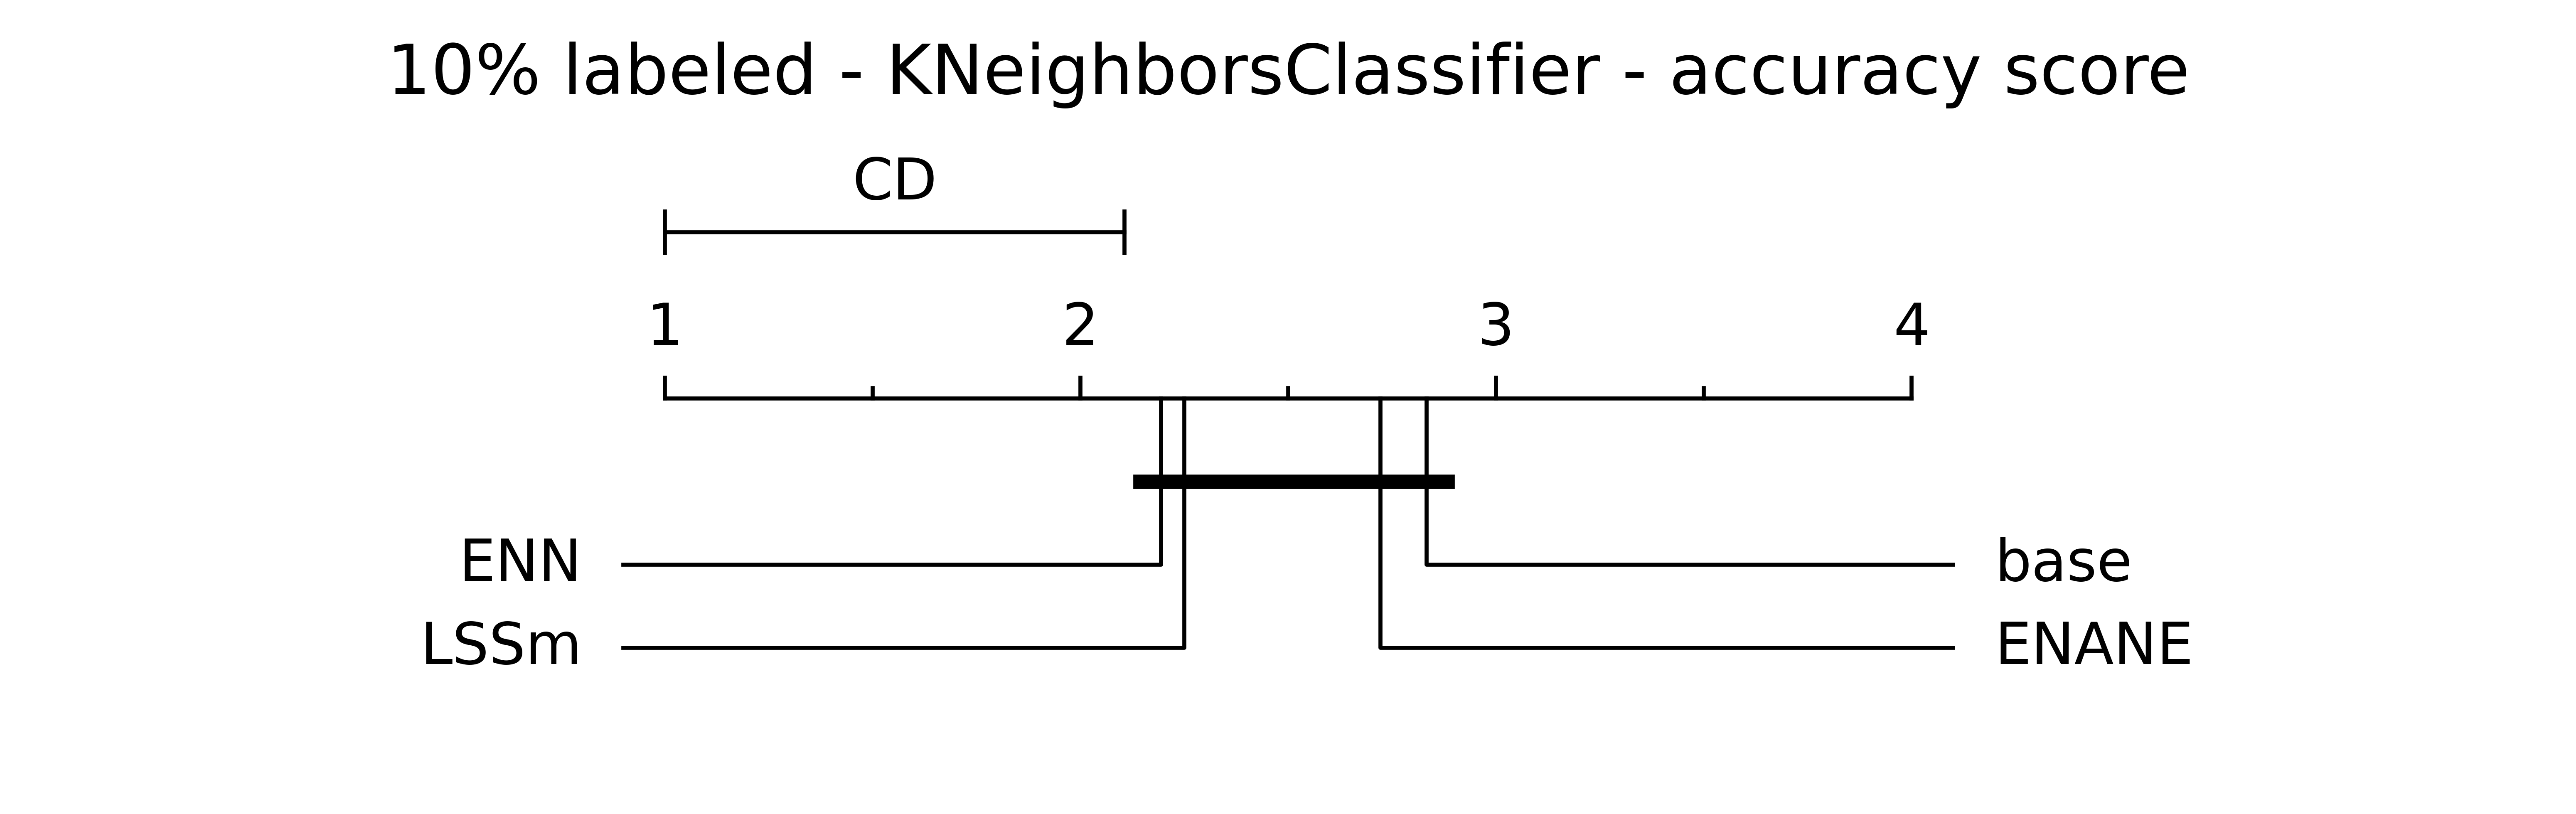
\includegraphics[width=\textwidth]{../img/memoria/aspectos-relevantes/knn-posthoc}
            \caption[]%
            {{\tiny Diagrama \textit{Critical Difference} para \textit{k-Nearest Neighbors}.}}    
            \label{fig:knn-posthoc}
        \end{subfigure}
        \hfill
        \begin{subfigure}[b]{0.475\textwidth}  
            \centering 
            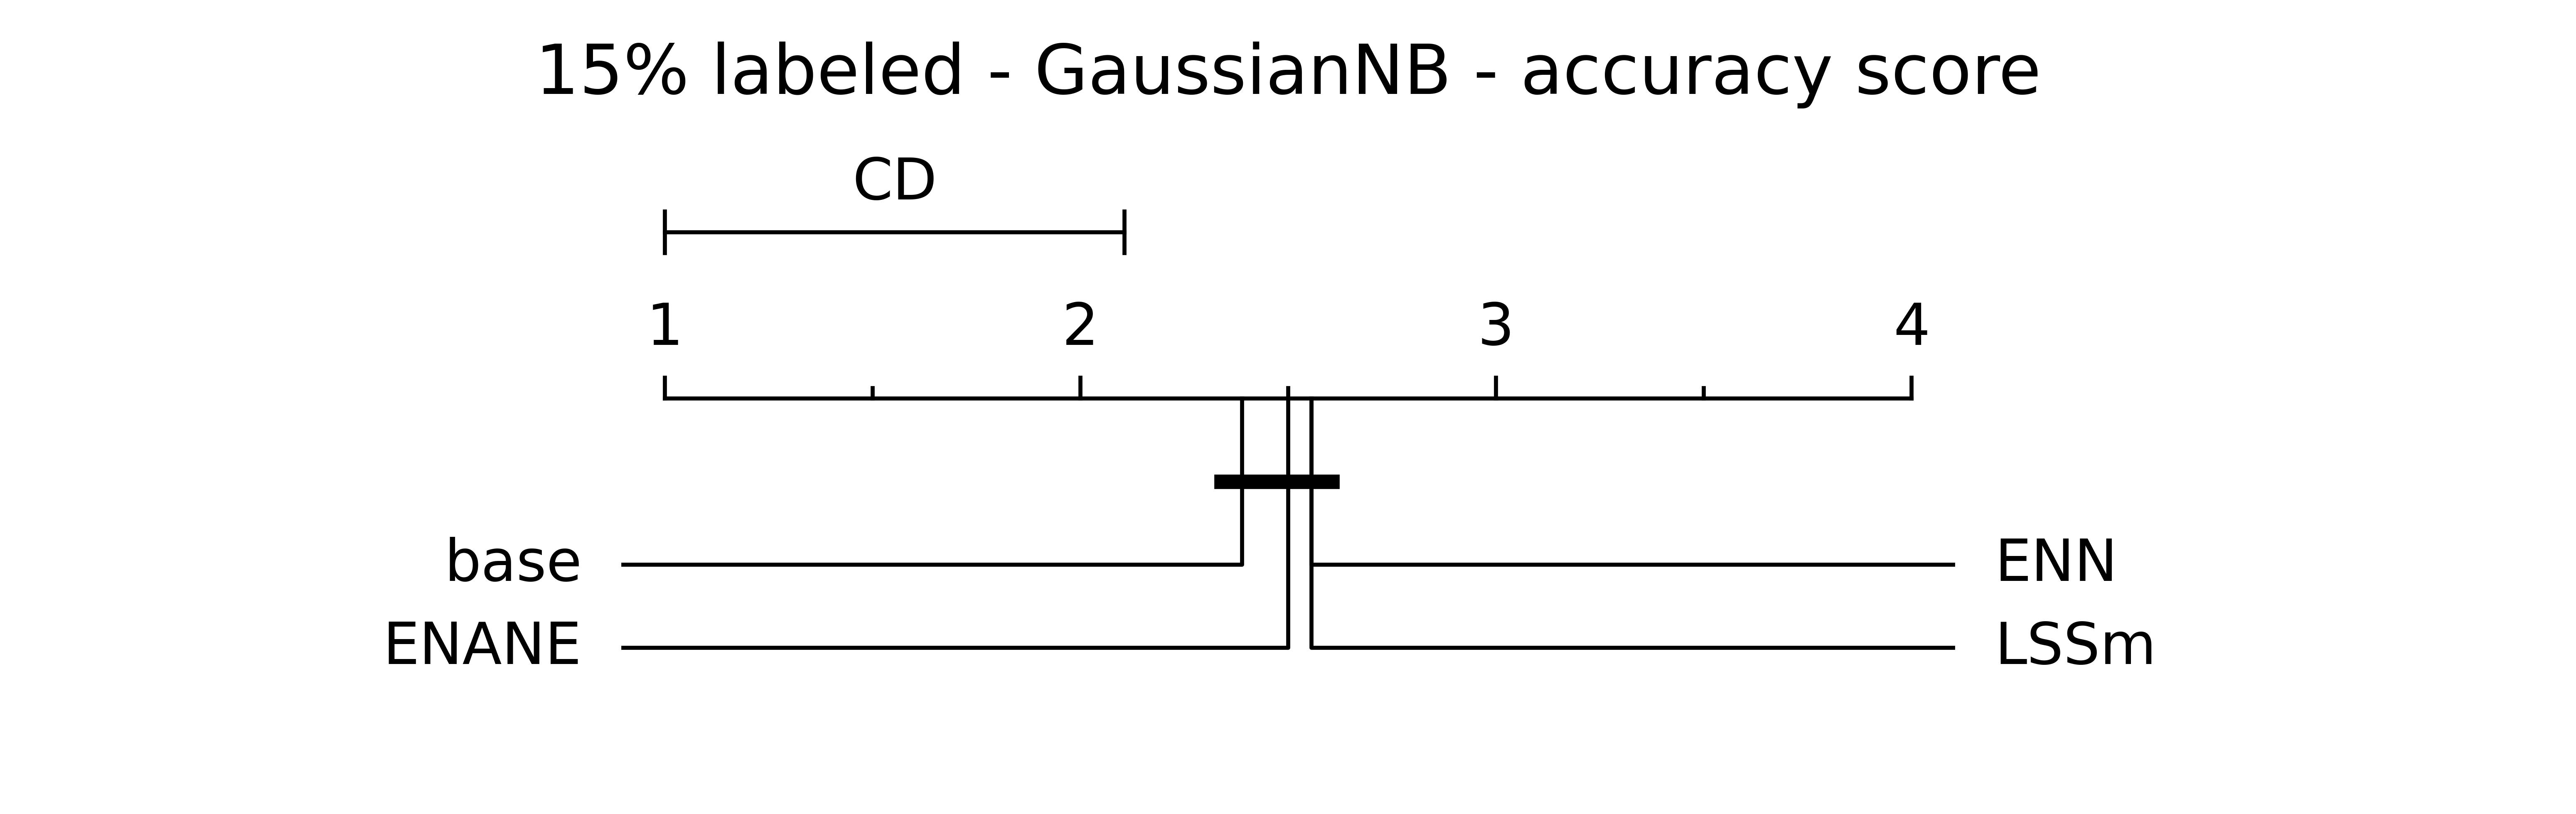
\includegraphics[width=\textwidth]{../img/memoria/aspectos-relevantes/gaussnb-posthoc}
            \caption[]%
            {{\tiny Diagrama \textit{Critical Difference} para \textit{Gaussian NB}.}}    
            \label{fig:gaussnb-posthoc}
        \end{subfigure}
        \vskip\baselineskip
        \begin{subfigure}[b]{0.475\textwidth}   
            \centering 
            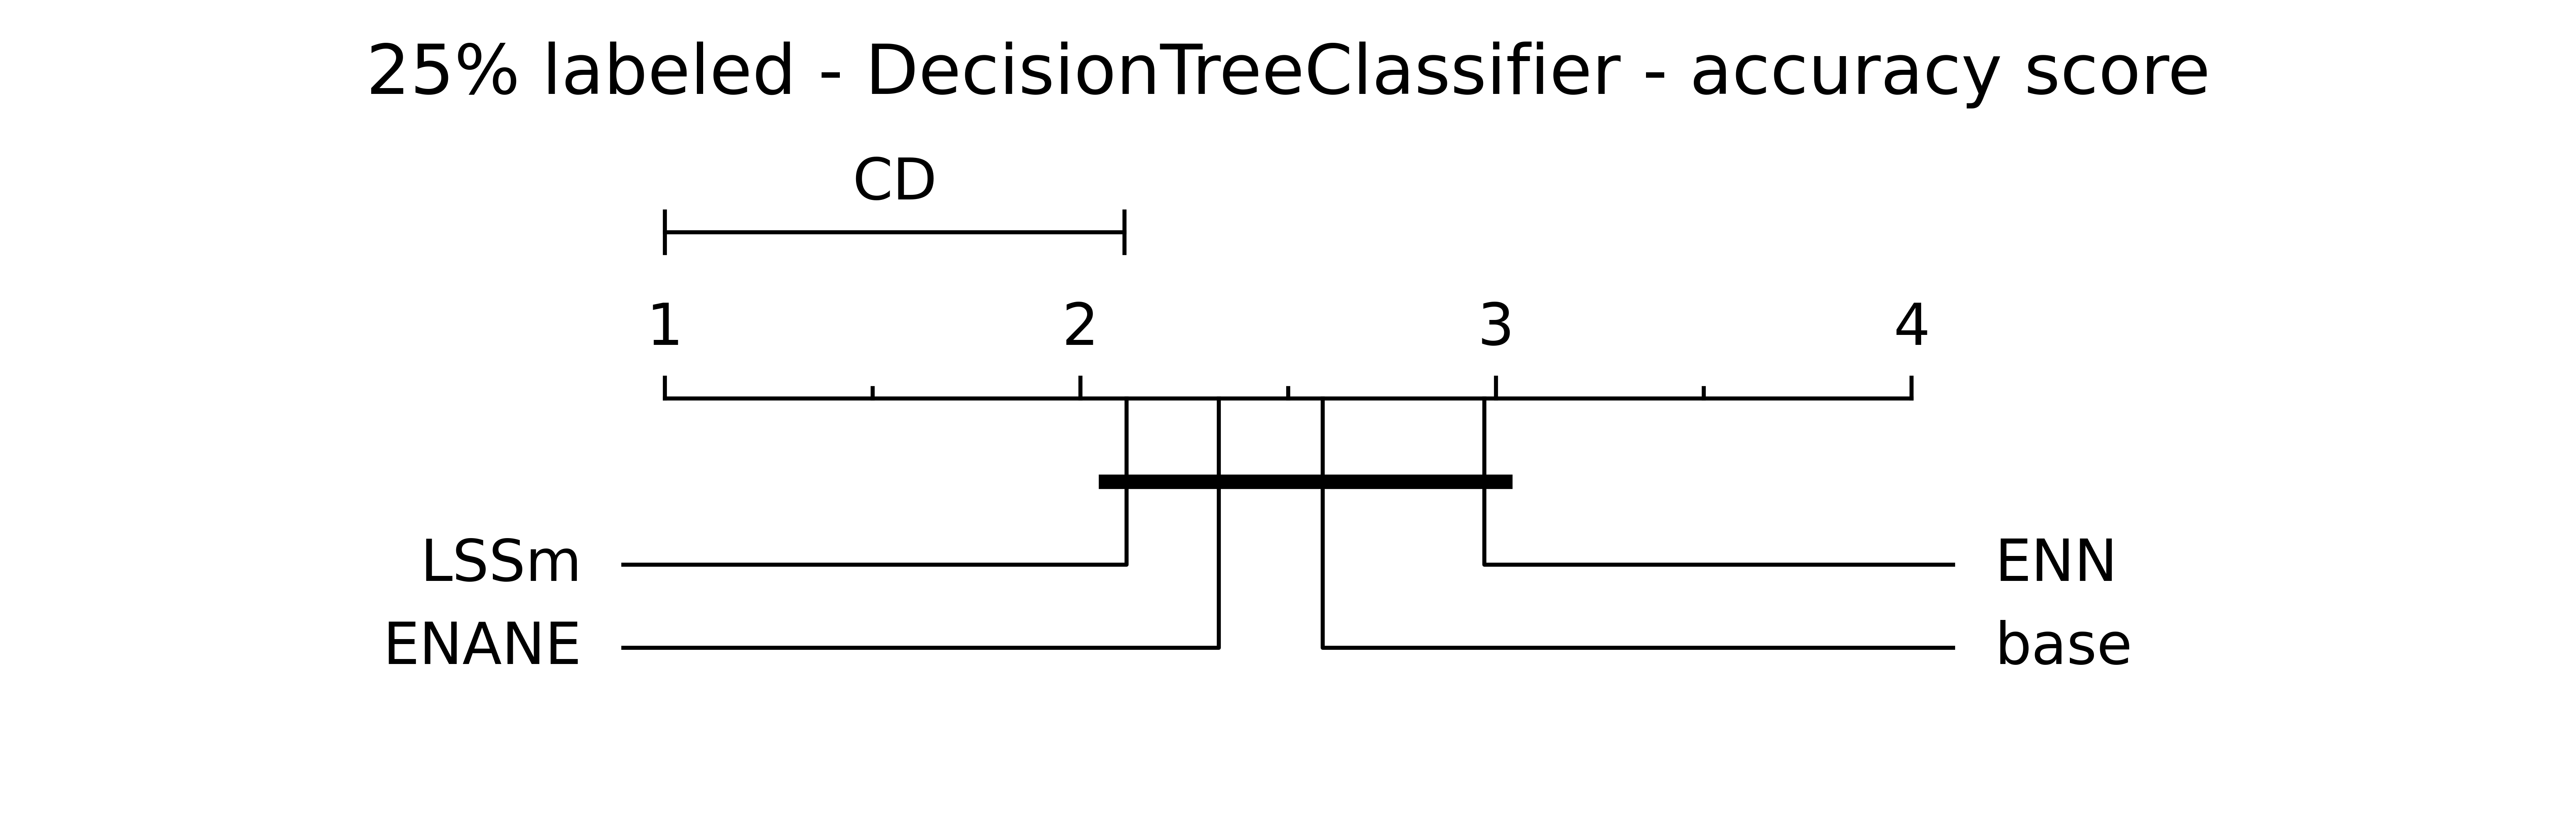
\includegraphics[width=\textwidth]{../img/memoria/aspectos-relevantes/tree-posthoc}
            \caption[]%
            {{\tiny Diagrama \textit{Critical Difference} para \textit{Decision Tree}.}}    
            \label{fig:tree-posthoc}
        \end{subfigure}
        \hfill
        \begin{subfigure}[b]{0.475\textwidth}   
            \centering 
            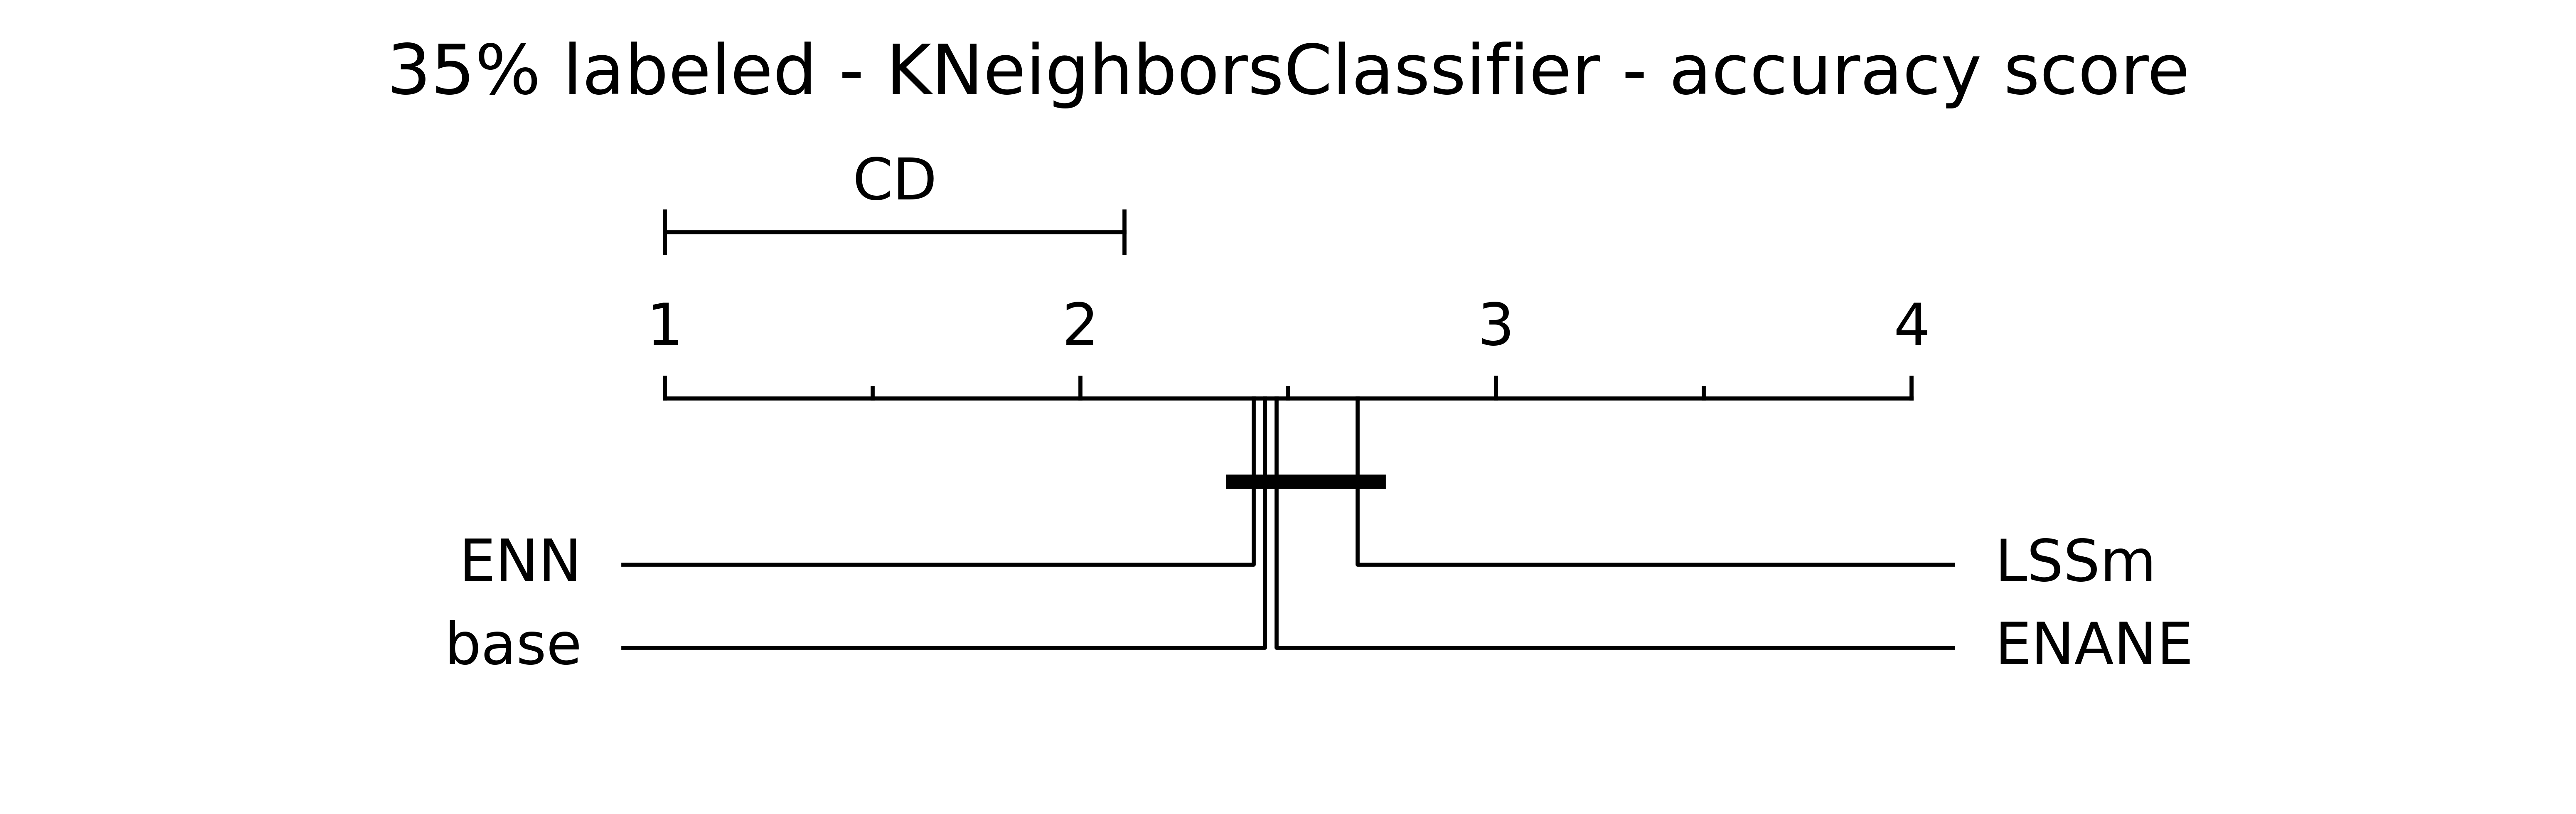
\includegraphics[width=\textwidth]{../img/memoria/aspectos-relevantes/knn2-posthoc}
            \caption[]%
            {{\tiny Diagrama \textit{Critical Difference} para \textit{k-Nearest Neighbors}.}}    
            \label{fig:knn2-posthoc}
        \end{subfigure}
        \caption[Diagramas de \textit{Critical Difference} para algunos porcentajes de etiquetado y clasificadores base utilizados.]
        {\small Diagramas de \textit{Critical Difference} para algunos porcentajes de etiquetado y clasificadores base utilizados.}
        \label{fig:CDs}
    \end{figure*}

\FloatBarrier
\subsection{Conclusiones}
Tal y como se apreciaba ya en la Figura~\ref{fig:exp-general}, no existen diferencias significativas entre los diferentes métodos de selección de instancias en relación con el aprendizaje semi-supervisado seguro. Los diagramas representando la Diferencia Crítica \ref{fig:knn-posthoc}, \ref{fig:gaussnb-posthoc}, \ref{fig:tree-posthoc}, y todos los demás no añadidos, no reportan en ningún caso un claro vencedor sobre los demás, para ningún clasificador base analizado. 

Estos resultados nos permiten llegar a la conclusión de que si bien los tiempos de ejecución son ligeramente inferiores en función del método de selección de instancias utilizado (en función de la <<agresividad>> con la que elimine instancias), no existe un ganador que nos permita asegurar que el uso de técnicas de selección de instancias con SSL lo haga más seguro.


